\documentclass{article}
\usepackage{tikz}
\usetikzlibrary{patterns}

\usetikzlibrary{hobby}
\begin{document}
	\begin{figure}[h]
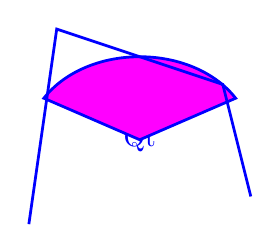
\begin{tikzpicture}
	\draw[color={rgb,255:red,000; green,000; blue,255}, draw opacity=1, line width=1pt, line cap=rect] (50pt ,-50pt) node {Qt};
	\draw[color={rgb,255:red,000; green,000; blue,255}, draw opacity=1, line width=1pt, line cap=rect, fill={rgb,255:red,255; green,000; blue,255}, fill opacity=1](50pt, -50pt) -- (84.6446pt, -34.9947pt) .. controls (77.7275pt, -26.0306pt) and (64.8027pt, -20pt) .. (50pt, -20pt) .. controls (35.1964pt, -20pt) and (22.271pt, -26.0313pt) .. (15.3541pt, -34.9964pt) -- (50pt, -50pt) -- cycle;
	\draw[color={rgb,255:red,000; green,000; blue,255}, draw opacity=1, line width=1pt, line cap=rect] (10pt, -80pt) -- (20pt, -10pt) -- (80pt, -30pt) -- (90pt, -70pt);
\end{tikzpicture}
		\caption{Latex TikZ Generator Example Drawing}
		\medskip\small\centering An Latex TikZ drawing created by the PaintLatex Generator Example provided with Qt.
	\end{figure}
\end{document}